\newpage
\subsection{[C] Sharing a list with a user}
In order to share a list with a user, hover on top of the \termine{bubble} that represents the list and click on the gear icon.

\begin{figure}[H]
  \centering 
  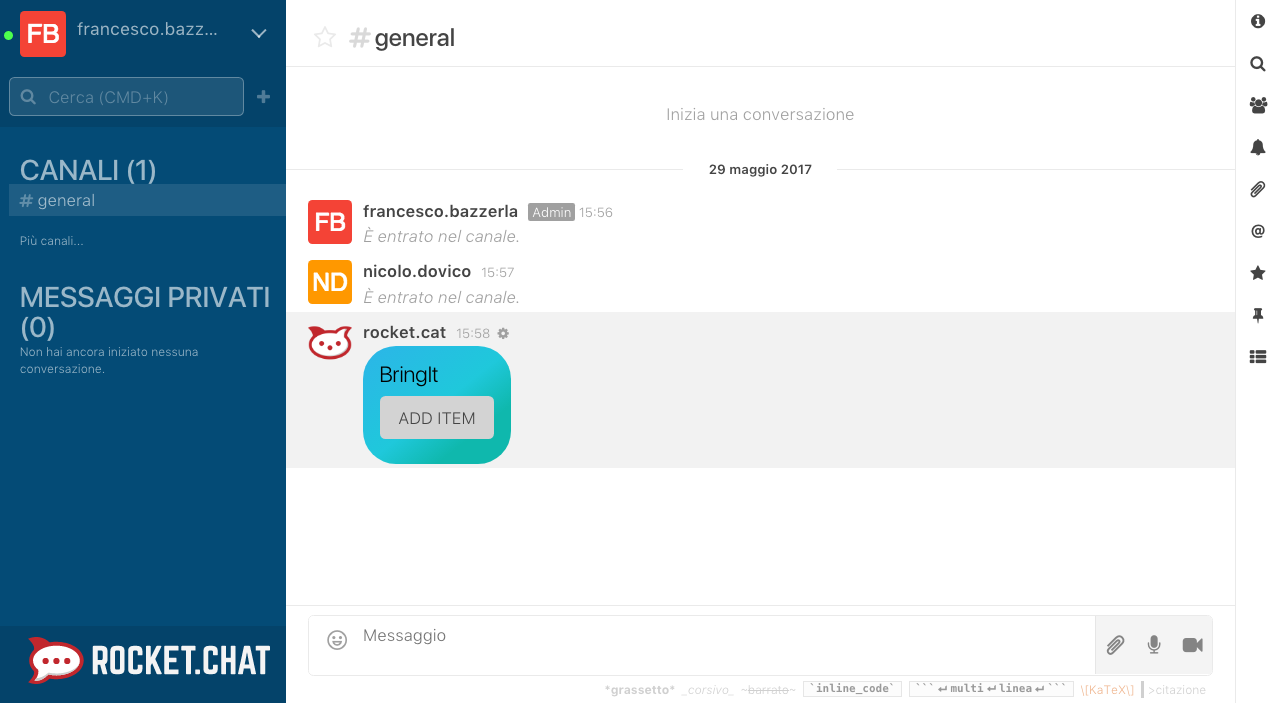
\includegraphics[width=\textwidth]{Sections/3-HowToUse/Images/bubble_options_button.png}
  \caption{Button to show the available list's actions.}
\end{figure}

From the various options that are available, click on the one with the user icon.

\begin{figure}[H]
  \centering 
  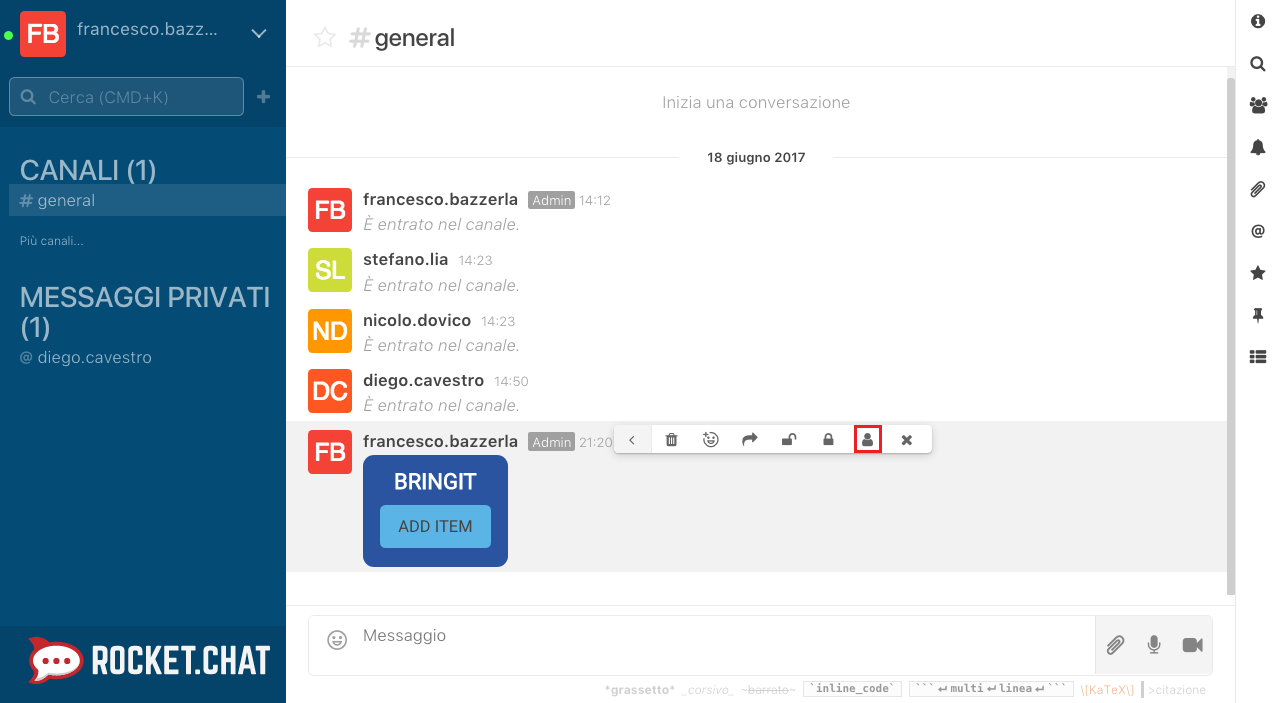
\includegraphics[width=\textwidth]{Sections/3-HowToUse/Images/bubble_option_share_user.png}
  \caption{Button to share the list with a specific user.}
\end{figure}

Once that the option has been clicked, the following popup will appear, showing the list of all the item that the list can be shared to.

\begin{figure}[H]
  \centering 
  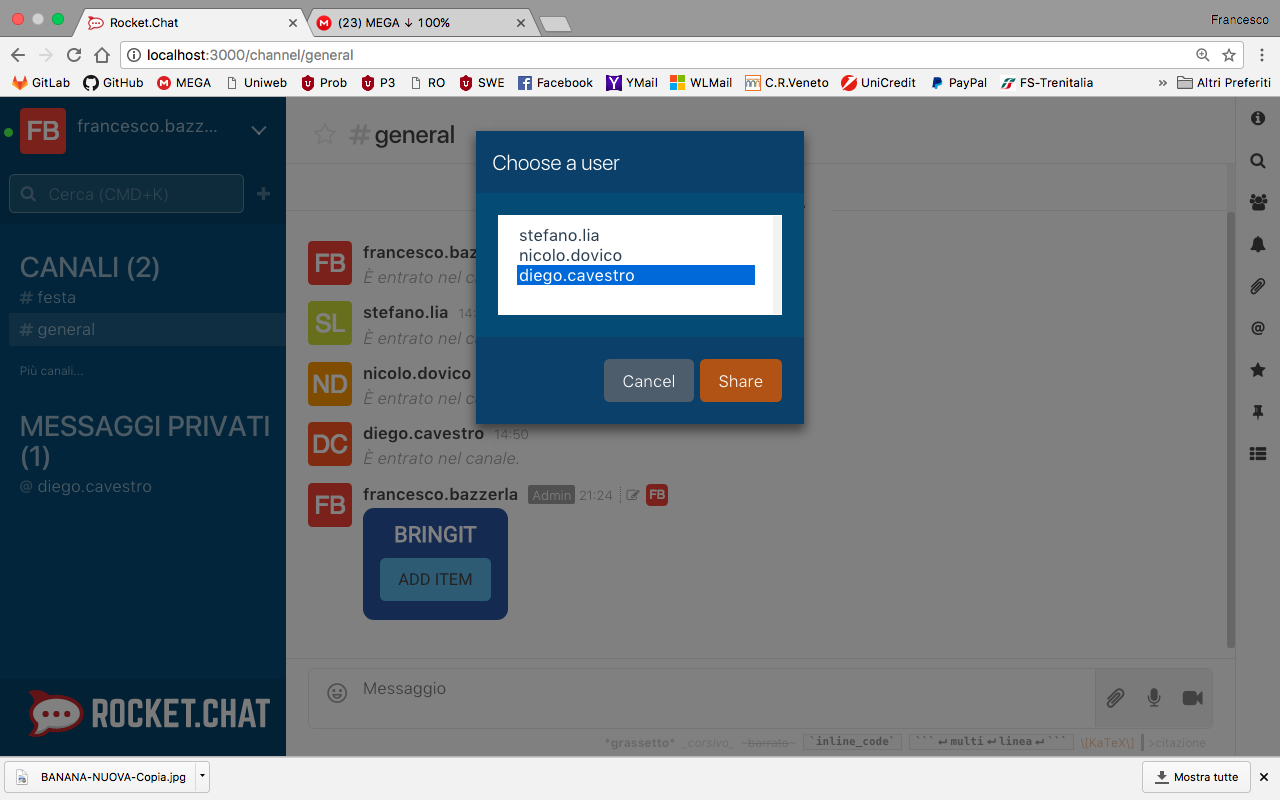
\includegraphics[width=\textwidth]{Sections/3-HowToUse/Images/popup_share_user.png}
  \caption{Popup showing the list of all the users to which is possible sharing a list.}
\end{figure}

Now, select the user you want share the list with and then click on \textit{"Share"}. \\
This will open the following popup, asking you to confirm the sharing action.

\begin{figure}[H]
  \centering 
  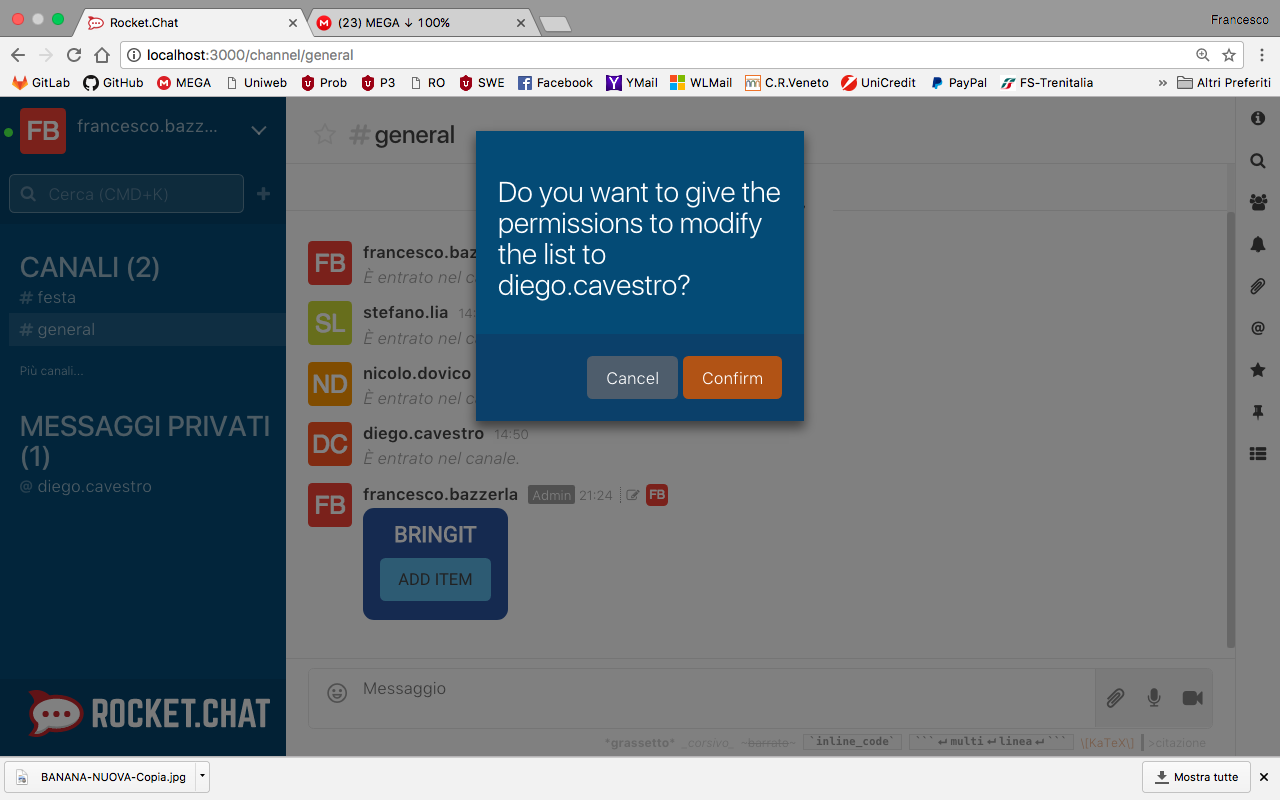
\includegraphics[width=\textwidth]{Sections/3-HowToUse/Images/popup_share_user_confirm.png}
  \caption{Popup to confirm the action to share the list with the selected user.}
\end{figure}

Once you have confirmed the sharing, the bubble will be sent inside the private chat with the user.

\begin{figure}[H]
  \centering 
  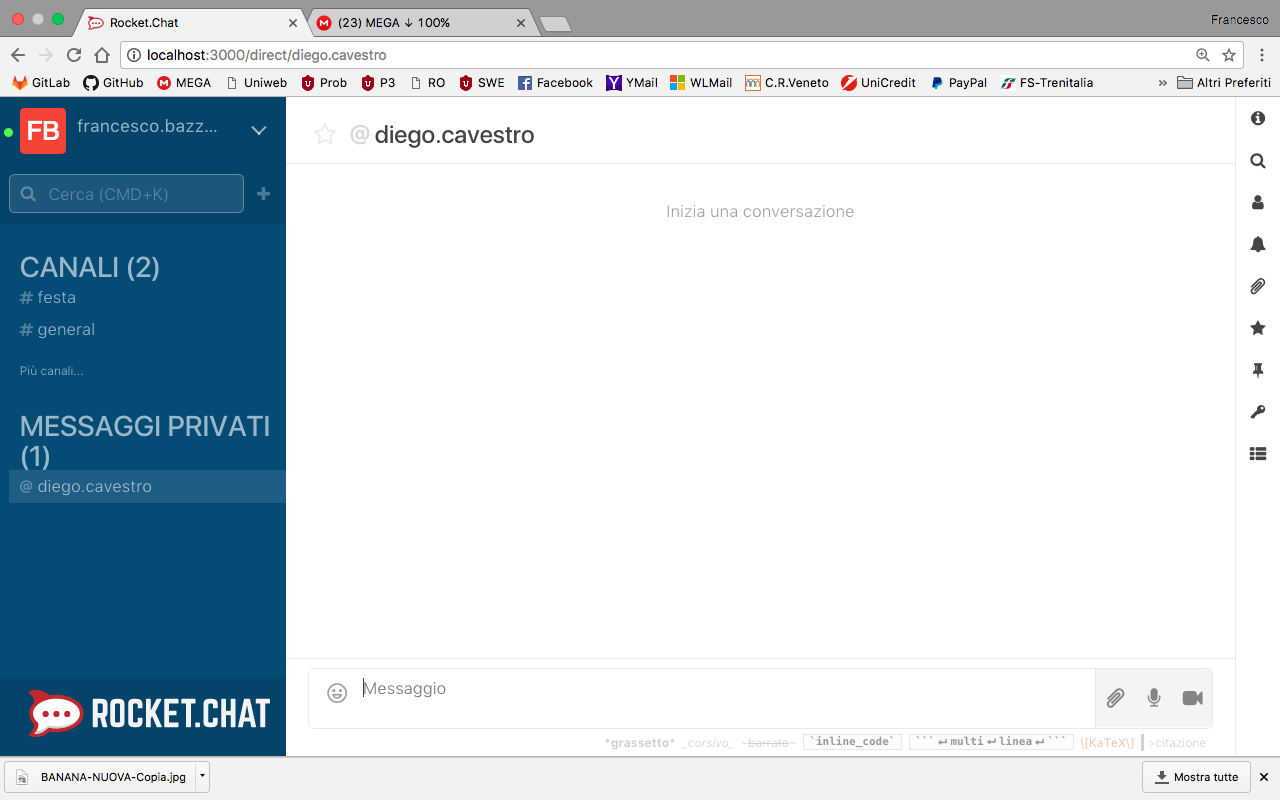
\includegraphics[width=\textwidth]{Sections/3-HowToUse/Images/share_user_before.png}
  \caption{Private chat with a user before sharing the list.}
\end{figure}

\begin{figure}[H]
  \centering 
  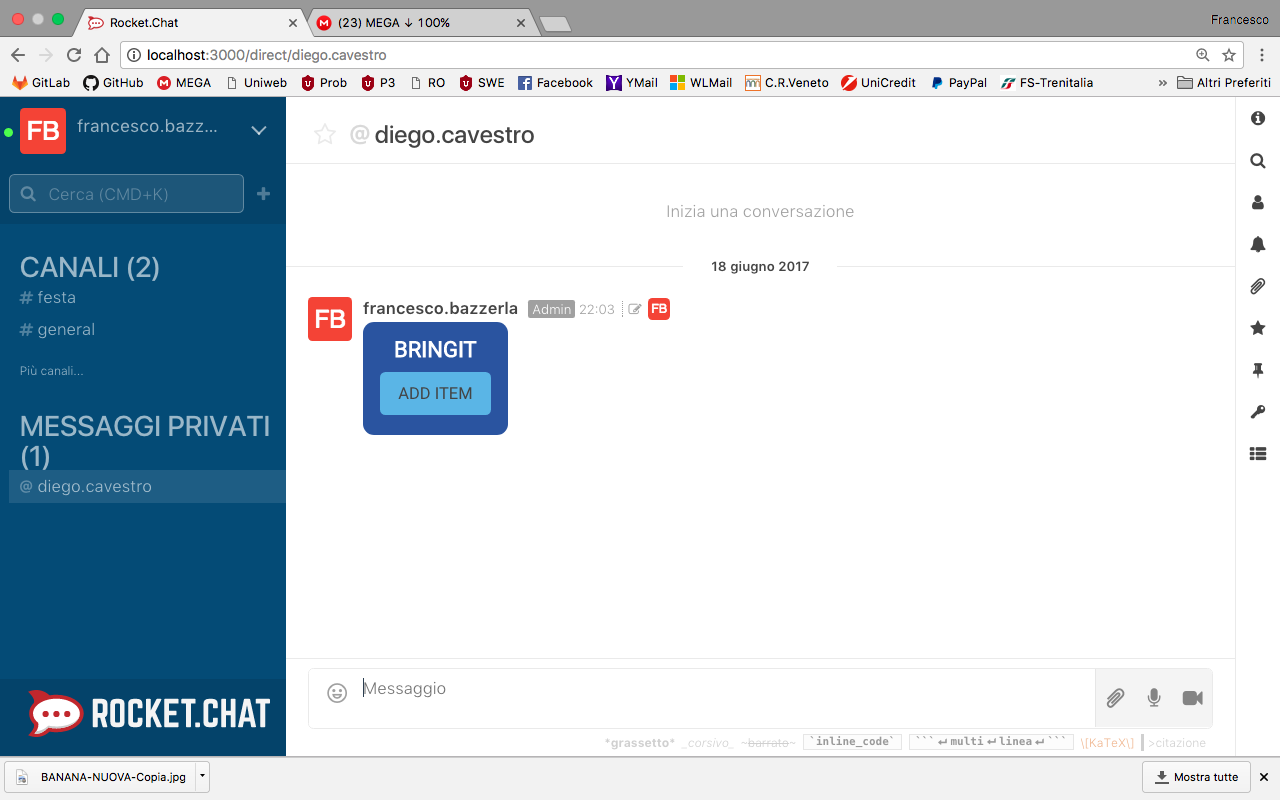
\includegraphics[width=\textwidth]{Sections/3-HowToUse/Images/share_user_after.png}
  \caption{Private chat with a user after sharing the list.}
\end{figure}


